\subsection{OB-13 (ASB)}
Bezpečnost bezdrátových sítí technologie Wi-Fi. Bezpečnostní standardy WEP, WPA, WPA2 a WPA3.

\begin{itemize}
	\item médium přenosu je prostor, tedy je to sdílené médium
	\item přenos elektromagnetickým vlněním v radiových frekvencích (20 kHz --- 300 GHz)
	\item využívá se CSMA/CA (carrier sense medium access / collision avoidance)
	\item 13 standardních pásem + 1 nestandardní cca kolem 2,4 GHz (šířka pásem cca 22 MHz, jsou odsunuté od sebe cca o 5MHz, tedy se překrývají částečně)
	\item struktura WiFi rámce:
	
	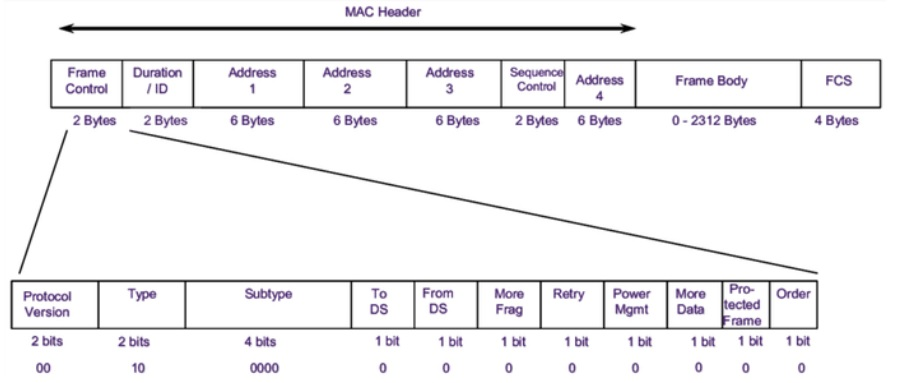
\includegraphics[width=0.8\textwidth]{img/OB-13_0.jpg}
	
	\item 4 různé MAC adresy s různými rolemi podle typu rámce:
	
	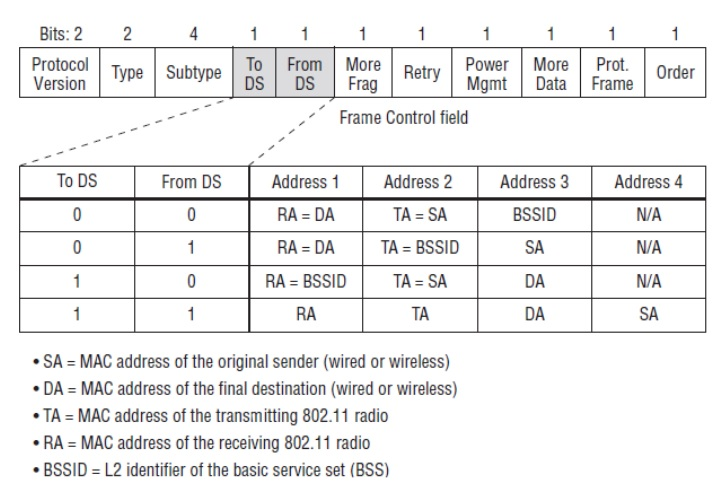
\includegraphics[width=0.8\textwidth]{img/OB-13_1.jpg}
	
	\item druhy rámců: management, control (RTS/CTS --- request to send, clear to send --- pro kontrolu toku dat), data
	
	\item management rámce
	\begin{itemize}
		\item Association request/response (žádost o připojení / odpověď)
		\item Reassociation request/response (znovupřipojení)
		\item Probe request/response (vyhledávání sítí, buď konkrétního SSID nebo všech)
		\item Beacon (ohlašování se --- vysílá se v pravidelných intervalech z AP, oznamuje jaké SSID jsou dostupná, spolu s konfigurací sítě)
		\item Authentication (proces pro ověření, zda je stanice schopna se připojit)
		\item Disassociation (bez odpovědi --- oznámení o odpojení)
		\item Deauthentication (resetuje stav připojení stanice)
		\item Action (vyvolají nějakou akci, lze pod to schovat nějaké nové typy rámců)
		\item Timing Advertisement (dnes se nepoužívá, předpokládáné využití v komunikaci se zařízeními co nemají vlastní čas)
	\end{itemize}
\end{itemize}

\subsubsection*{WEP}
\begin{itemize}
	\item Wired Eqivalent Privacy
	\item zastaralý bezpečnostní standard, vydán v roce 1999
	\item autentizace --- stanice pošle request, AP pošle v plaintextu challenge, stanice zašifruje a pošle reponse, dostane zpět potvrzení
	\item RC4 pro šifrování, CRC32 pro integritu
	
	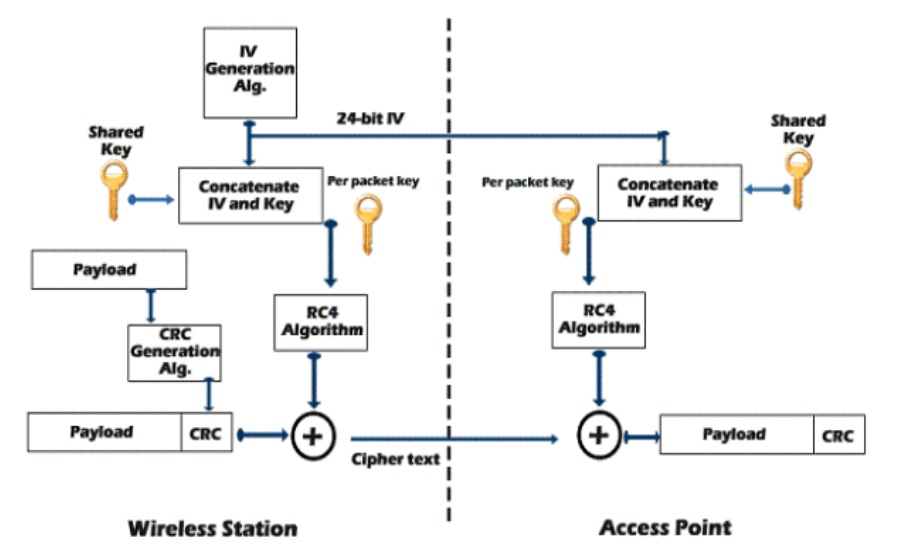
\includegraphics[width=0.8\textwidth]{img/OB-13_2.jpg}
	
	\item problémy:
	\begin{itemize}
		\item sdílený klíč je používán pro autentizaci i pro šifrování dat
		\item znovupoužití keystreamu
		\item sdílený klíč se nemění (nebo jen málo často)
		\item IV se sdílí veřejně, je možné zachytit opakující se IV
		\item teoreticky 24 bitů IV, prakticky kolize po cca 5000 paketech
	\end{itemize}
\end{itemize}

\subsubsection*{WPA/WPA2}
\begin{itemize}
	\item Wi-Fi Protected Access
	\item různé módy autentizace --- personal (WPA-PSK, pre-shared key) nebo enterprise
	\item 4-way handshake (WPA/WPA2)
	
	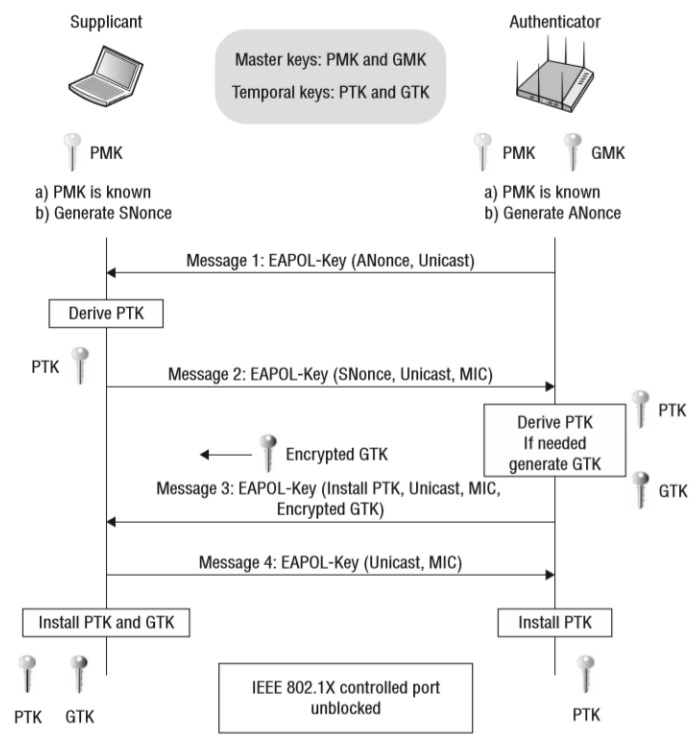
\includegraphics[width=0.7\textwidth]{img/OB-13_3.jpg}
	
	\begin{itemize}
		\item PSK --- pre-shared key
		\item PMK --- pairwise master key = PBKDF2(HMAC-SHA1, PSK, SSID, 4096, 256) --- Password-Based Key Derivation Function 2
		\item PTK --- pairwise transit key = PRF(PMK, "Pairwise Key Expansion", MAC1, MAC2, nonce1, nonce2) --- Pseudo Random Function
		\item ANonce --- náhodné číslo AP
		\item SNonce --- náhodné číslo stanice
		\item případně GMK, GTK ---  Group Master/Temporal Key
	\end{itemize}
	\item problém s handshake --- lze zachytit a offline hádat klíč díky MIC --- Message Integrity Code spočítaný pomocí PTK
	\item šifrování v WPA --- TKIP (Temporal Key Integrity Protocol), založený na RC4
	\item šifrování v WPA2 --- CCMP (Ctr mode with CBC-MAC Protocol), založený na AES
\end{itemize}

\subsubsection*{WPA3}
\begin{itemize}
	\item obsahuje forward secrecy
	\item PMK se nevytváří z PSK
	\item vyřešený problém s handshake:
	
	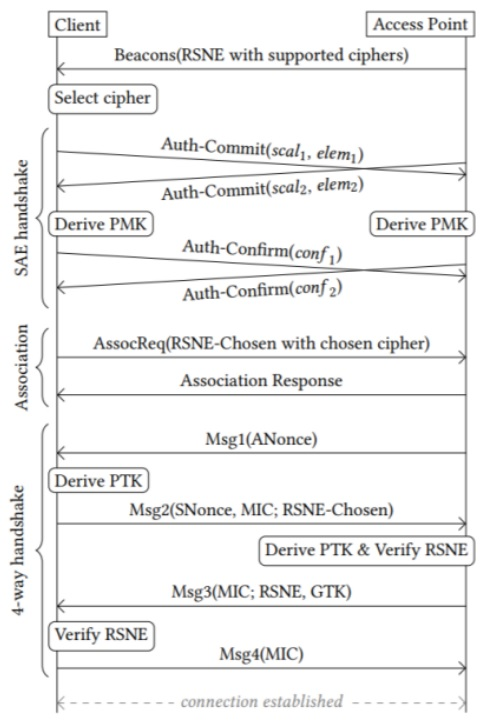
\includegraphics[width=0.6\textwidth]{img/OB-13_4.jpg}
	
	\item SPEKE --- Simple Password Exponential Key Exchange
	\begin{itemize}
		\item A a B si dohodnou prvočíslo $p$, hash funkci $H$ a sdílené heslo $P$ (může být PSK u personal wifi)
		\item oba spočítají generátor $G = H(P)$
		\item následuje Diffie-Hellman výměna, spočítají společný klíč $K = |G^{a \cdot b}|_p$
	\end{itemize}
	\item existuje upravená verze "Dragonfly" využívající eliptických křivek
	\item stále lze na Wi-Fi útočit, lámat slabá hesla, zkoušt rainbow-tables pro nejznámější SSID, downgrade attack...
\end{itemize}